\subsection{Command (\textit{o Action, Transaction})}
\label{command}

\textbf{Scopo}: Comportamentale \\
\textbf{Raggio d'azione}: Oggetti

\paragraph{Definizione} Il pattern Command incapsula una richiesta in un oggetto, consentendo di parametrizzare i client con richieste diverse, accodare o mantenere uno storico delle richieste e gestire richieste cancellabili.

\begin{figure}[H]
    \centering
    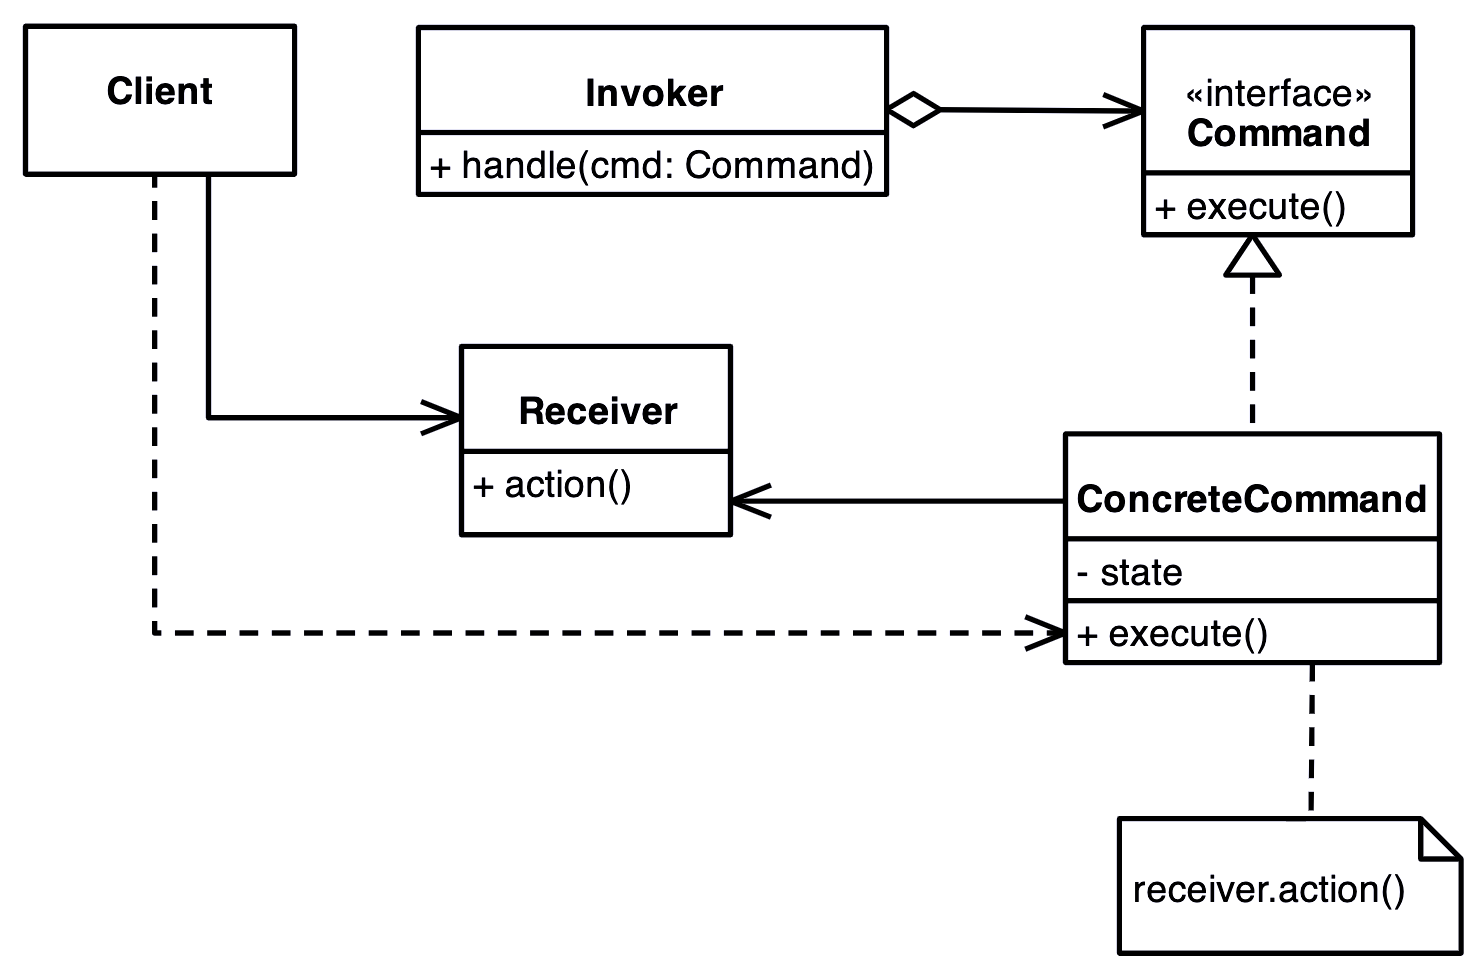
\includegraphics[width=1\linewidth]{assets/pattern/command/command-struttura.png}
\end{figure}

\paragraph{Struttura} Il pattern Command è composto da:
\begin{itemize}
    \item \textbf{Command}: dichiara un’interfaccia per l’esecuzione di un’operazione generica. 
    \item \textbf{ConcreteCommand} (PasteCommand, OpenCommand): definisce un legame fra un oggetto destinatario e un’azione. Implementa il metodo execute() invocando il metodo (i metodi) corrispondente sul Receiver. 
    \item \textbf{Client} (Application): crea un’istanza concreta di Command e ne imposta il Receiver. 
    \item \textbf{Invoker} (MenuItem): chiede a Command di portare a termine la richiesta 
    \item \textbf{Receiver} (Document, Application): conosce il modo di svolgere le operazioni associate a una richiesta. Qualsiasi classe può essere vista come Receiver.
\end{itemize}

\begin{figure}[H]
    \centering
    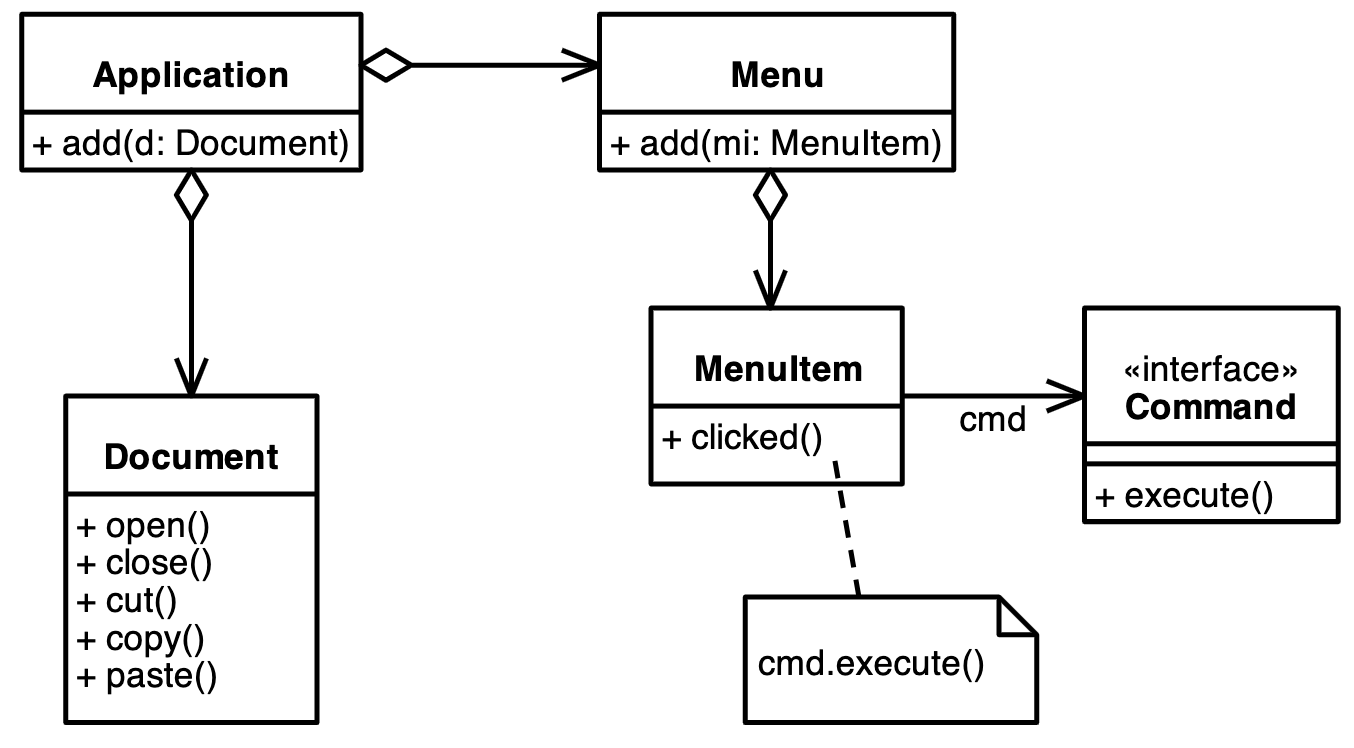
\includegraphics[width=1\linewidth]{assets/pattern/command/command-esempio.png}
\end{figure}

\paragraph{Conseguenze} Command disaccoppia l’oggetto che invoca un’operazione da quello che conosce come portarla a termine. 
Gli oggetti Command sono oggetti a tutti gli effetti, possono essere manipolati ed estesi con un qualsiasi altro oggetto. 
È possibile comporre più comandi in un comando composito.
In generale, i comandi compositi sono un’istanza del pattern Composite.
Risulta facile aggiungere nuovi comandi poiché non è necessario modificare le classi esistenti

\begin{figure}[H]
    \centering
    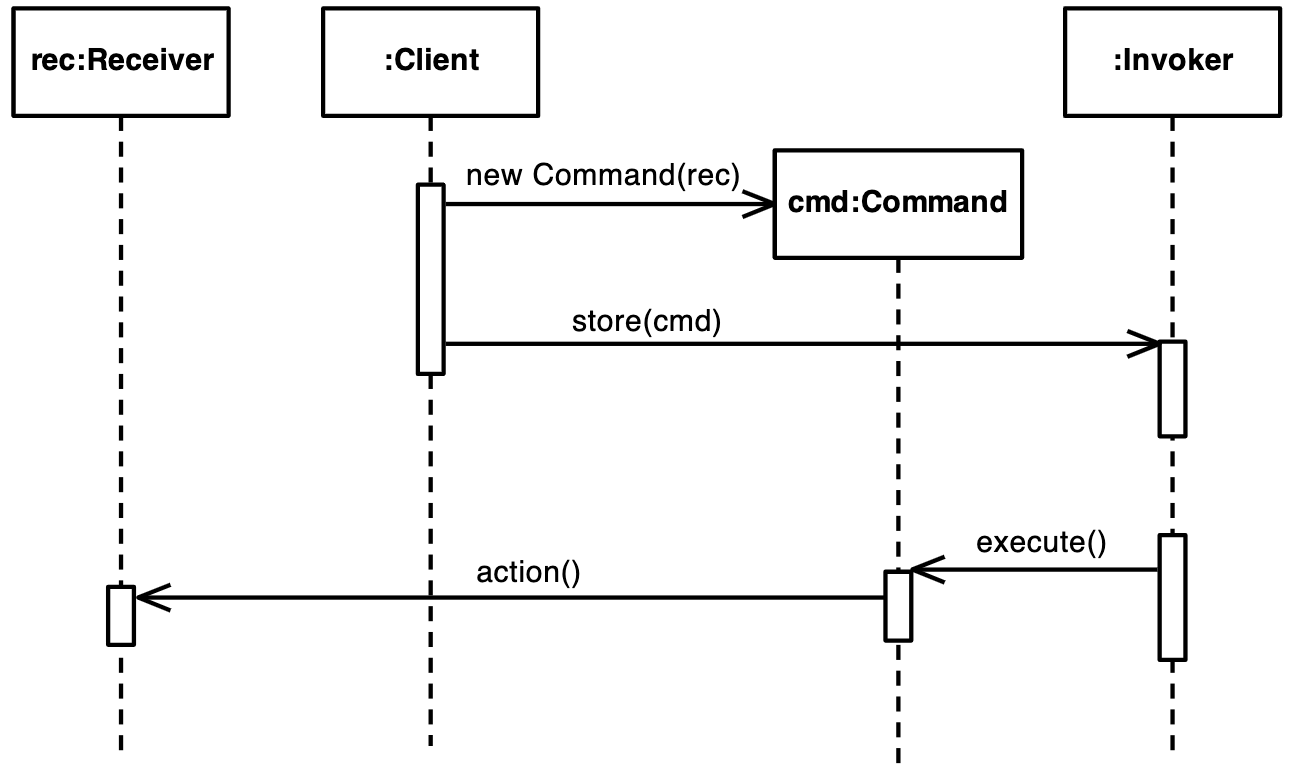
\includegraphics[width=1\linewidth]{assets/pattern/command/command-sequence.png}
    \caption{Sequence Diagram del pattern Command}
\end{figure}



\newpage